\chapter{实验平台设计与开发}

上一章介绍了使用定性研究方法进行的一次用户研究,但是,定性研究它只能给出一个大致的改进的思路,并不是一个量化的设计方面的解决方案,
例如具体应该怎么设计系统才能更好的增加系统的透明性,这需要进一步的设计并进行交互实验。
此外,在上一章我们提到了基于技术探针的交互实验流程,它的主要特点如是需要一个快速迭代的原型系统,不断根据用户的反馈进行版本迭代。

在后续的研究中,我们需要对大量线上用户进行批量的研究,为了方便后续的实验,我们需要设计一个全新的系统架构,解决两个方面问题:

\begin{enumerate}
    \item 设备多样性带来的系统可用性的问题。
回顾绪论中提到的日常用户使用场景的特点之一是设备多样性。从实地调研的发现中可以知道,因为部分用户设备老旧的问题以及系统平台的差异,设备多样性的问题已经严重影响了大量用户的使用,我们需要从系统设计方面解决这个问题。

    \item 如何提高实验的规模和效率。在类似场景下,我们需要一个可以快速对人脸模型进行人机交互实验的平台,方便后续的具体的交互研究,同时支持大批量地线上开展实验。
\end{enumerate}

% \subsubsection{技术探针实验流程特点}
% 在上一章我们提到了


% 根据上面的调研结果,可以改进的方面有很多。但是从用户日常使用的角度,影响用户持续使用最大的问题是可用性的问题和理解的问题。

% 可用性的解决方案主要分为两块:一个是提高系统的可用性;另一个是重新设计用户友好的交互界面,提升交互的体验。增强用户理解则是通过加入透明性。


\section{基于技术探针的实验平台设计}
% \subsection{技术探针系统设计}
% 作为我们技术探针的云中医只有Android版本,核心诊断和打分算法使用c++编写, 分类模型为OpenCV模型。
% 在具体实现方面,将所有OpenCV格式模型打包到Android安装包中,在Android平台通过Native方法调用动态链接库的方式完成诊断。

% 这种非跨平台的实现,有一个明显的缺点就是系统的稳定性需要考虑的用户各种设备环境。在用户调研过程中,很多用户曾经反馈在使用过程中无法完成诊断或者闪退。

\subsection{设计理念}

% 在这个平台做透明性的研究,通用实验平台的设计和搭建
% 用户操作记录管理,为了实验,
% 开关控制,

% 后续的实验流程 TODO:来一个图

% 为什么只用它的这个?

为了支持后续的交互研究实验,经过调研和讨论,该平台需要提供一下几种特性或者功能:

\begin{enumerate}
    \item 模型管理。新的人脸相关的模型,需要能够快速接入系统。当前人工智能技术发展迅速,不断有新的模型出现。为了让新的模型能够快速接入,系统需要对模型进行抽象,能够快速将模型应用到系统,以便开展实验工作。

    \item 任务分配与调度。从用户面部等信息到得出面诊的最终结果,是一个相对比较复杂的任务,需要经过一系列的处理和模型调用。通过对面诊任务拆分成多个子任务,可以提高系统的稳定性。
任务拆分之后,系统需要实现多任务在多平台上的分配与调度。

    \item 用户操作记录管理。用户的操作记录对分析用户行为非常重要,系统需要记录用户在客户端的所有行为,方便之后分析用户的行为。操作记录的在线管理,导出到文件等功能,便于离线和在线查看用户操作记录。

    \item 问卷关联。可定制化问卷在交互试验中可以完成个人信息采集,资格测验,前后对比等功能。
我们采用第三方问卷(如问卷星\footnote{https://www.wjx.cn/})的形式完成可定制化问卷,因此系统需要支持第三方问卷系统跳转完成自动登录,以及问卷数据和用户操作记录信息关联的功能。
\end{enumerate}


\subsection{方案比较}
在实现原型的架构方面,经过考虑有以下方案:

\subsubsection{方案一}
Android平台编写一套代码,通过JNI调用动态链接库的方式调用模型; IOS编写一套代码,通过swift语言调用链接库的方式调用模型; Web平台重新编写一套代码,通过接口调用的方式调用模型。

\begin{itemize}
    \item 优点: 模型放在客户端本地,没有网络也可以完成诊断。

    \item 缺点: 需要重新编写Android、IOS和Web平台代码,需要同时维护三个平台的代码,保持功能界面的一致性。移动端平台模型是本地调用,不方便统一管理。模型本地调用需要考虑客户端的系统平台和设备性能,
这种非跨平台的实现,系统的稳定性需要考虑的用户各种设备环境。
\end{itemize}

在用户调研过程中,很多用户曾经反馈在使用过程中无法完成诊断或者闪退,这种方式的缺点已经严重影响了部分用户的正常使用,也限制了我们实验招募的用户群体的范围。

\subsubsection{方案二}

采用C/S架构,全部重写。IOS,Android以及Web客户端使用一套H5代码, 处理逻辑在服务端实现,模型独立服务化,通过Http接口的方式调用。

\begin{itemize}
    \item 优点: 客户端使用一套H5代码,维护方便。模型部署在服务器,无泄密风险,可以统一管理(统计调用次数,记录错误日志等),方便实现高可用。支持热更新,即H5可以在不更新客户端的情况下更新H5文件完成功能的更新。

    \item 缺点: 依赖网络稳定性和模型服务的稳定性,代码编写的工作量稍大, 需要另外实现模型服务化和服务端平台。
\end{itemize}

为了适应各种类型的交互研究,客户端版本更新的速度会非常快,同时我们希望用户的设备类型不能成为障碍,跨平台是较好的解决方法。
方案一的缺点会导致后续的维护成本过大且系统不稳定,考虑到后续需要实现一个灵活可拓展的实验平台,而方案二更符合前面提到的设计理念,且更方便拓展成分布式的系统,本文最终采用方案二。

\subsection{系统简介}
\begin{figure}[ht]
    \centering
    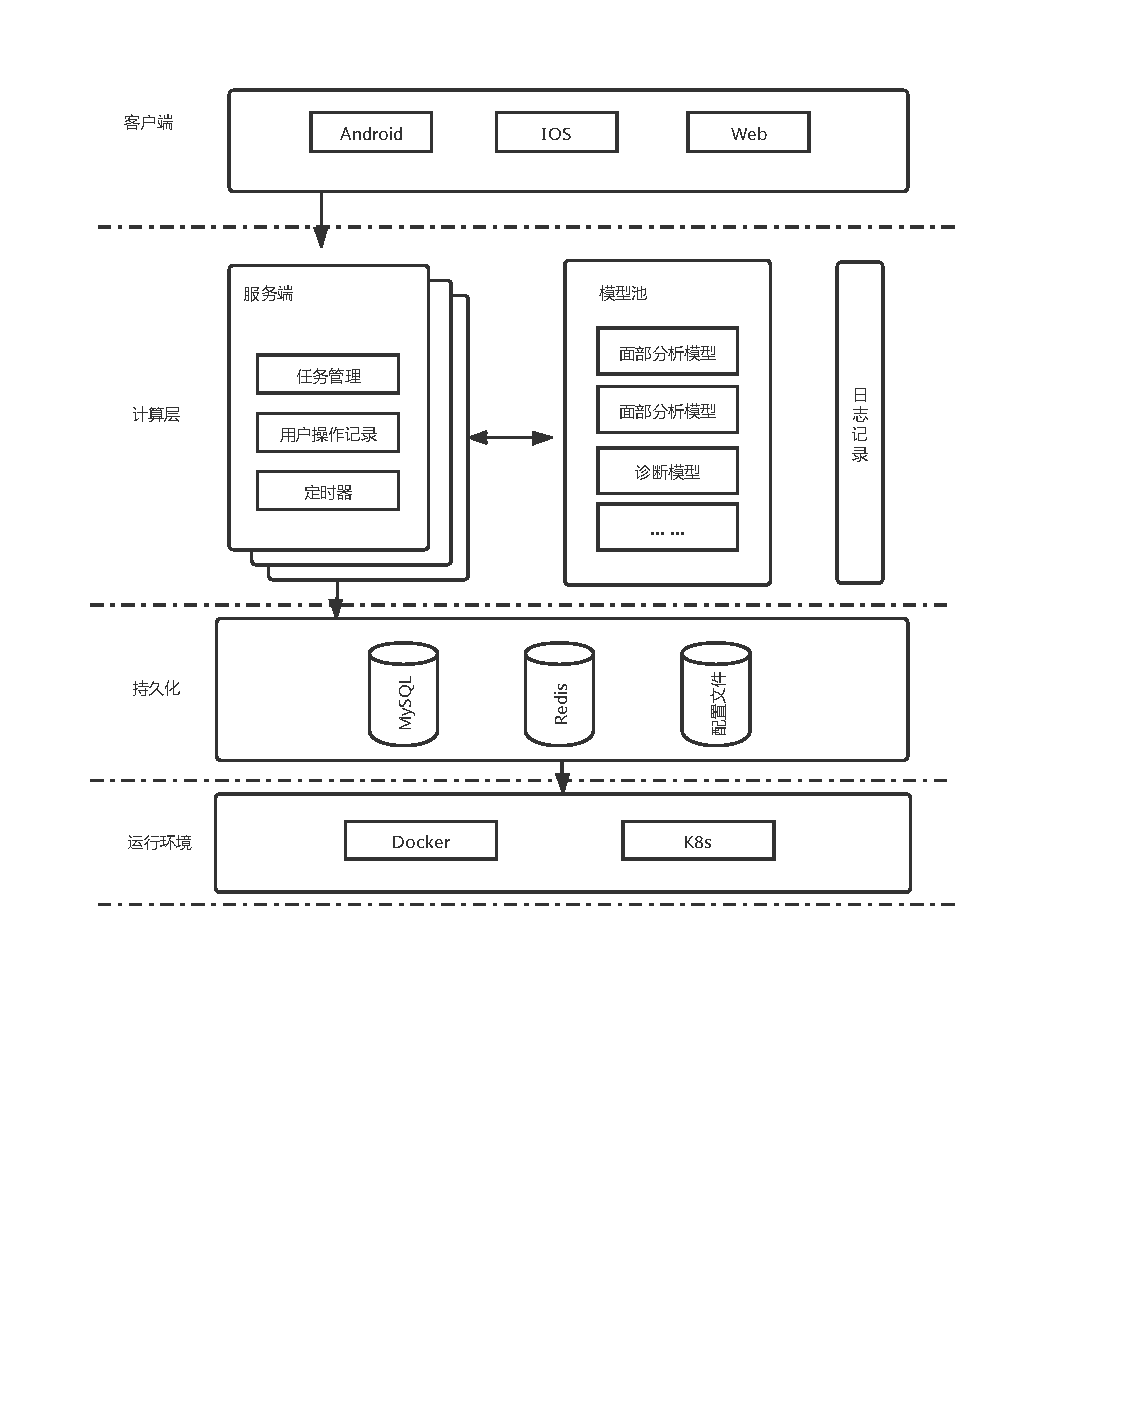
\includegraphics[width=15cm]{images/system2.pdf}
    \caption{跨平台系统设计}
    \label{fig:system}
\end{figure}

如图\ref{fig:system}所示,系统整体运行在容器环境下,使用Redis和MySQL作为持久化工具,主要分为三部分:服务端和客户端,算法模型通过容器的方式(docker\footnote{https://www.docker.com/}、kubernetes\footnote{https://kubernetes.io/})服务化成模型池。

客户端包括Android、IOS和Web平台的客户端,与用户交互密切相关,负责用户面诊的流程已经数据上传,通过请求服务端的接口完成面诊和记录用户的操作信息;
服务端通过调用模型池的相关服务,为客户端提供接口服务。其中静态页面的服务通过nginx提供,服务端则使用Django作为开发框架;
模型池是指在容器环境下通过容器服务化的方式下所有可用的模型服务的统称,为服务端提供计算服务,完成面部图片分析,舌部图片分析等任务。
大多数模型格式为二进制可执行文件或者本地模型文件的形式,为了方便服务端调用,需要对其进行服务化。

服务化指的就是将算法模型,打包成可调用的服务。其中本文的模型服务化通过Flask框架实现,每一个模型的服务都可以对应服务端中的一个计算任务。
服务端在任务管理模块中定义了任务的输入输出格式,模型池中的服务只要保持格式一致就可以保证服务端能够顺利调用对应的模型服务。

一次诊断的大致流程如下:用户通过客户端,上传图片或者回答问题,客户端则向服务端发起请求。
服务端收到请求之后,进行任务分配,对分配到任务的服务端实例,调用模型池中对应的模型完成特征提取或诊断打分,同时将数据持久化到mysql和硬盘中,然后把结果返回给客户端。
客户端收到服务端的结果后,进行结果的展示。

\section{模型池}
% 什么是模型池
本文提出一个模型池的概念,模型池由多个独立可用的模型服务构成, 通过http 接口调用完成和服务端的交互进行任务处理。

% 为什么要模型池
提出模型池的概念,是为了将模型和服务端独立,方便以后添加或删除模型。同时,将模型独立做成服务,可以动态增加模型运行的实例个数,提高计算能力和稳定性。


% \begin{figure}[h]
%     \centering
%     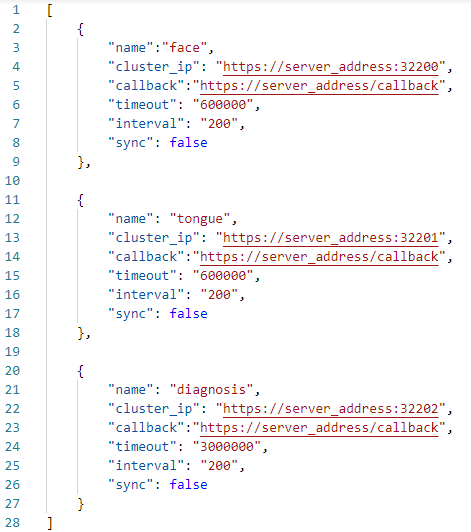
\includegraphics[width=15cm]{images/services2.png}
%     \caption{模型池配置}
%     \label{fig:services}
% \end{figure}

\begin{lstlisting}[language={Python}, title=services.json]
[
    {
        "name":"face",
        "cluster_ip": "https://server_address:32200",
        "callback":"https://server_address/callback",
        "timeout": "600000",
        "interval": "200",
        "sync": false
    }, 
    
    {
        "name": "tongue",
        "cluster_ip": "https://server_address:32201",
        "callback":"https://server_address/callback",
        "timeout": "600000",
        "interval": "200",
        "sync": false
    },
    
    {
        "name": "diagnosis",
        "cluster_ip": "https://server_address:32202",
        "callback":"https://server_address/callback",
        "timeout": "3000000",
        "interval": "200",
        "sync": false
    }
]
    
\end{lstlisting}

% 如何实现的
如services.json所示,模型池维护一个<模型类型, cluster ip> 的映射,记录可用的模型和调用地址, cluster ip是由k8s(kubernetes)提供的集群调用地址。记录通过json文件的格式,记录在本地文件中。
其中sync参数代表是否同步返回结果,如果设置成异步返回,则通过调用callback地址将结果回调给服务端。timeout字段用于预先设置服务的超时时间,由于不同的服务计算时间不同,可以根据模型的实际运行速度进行调整。
interval字段表示失败或者超时的重试间隔,默认设置为200毫秒。

服务的稳定性和高可用需要做到服务之间相互独立和多实例同时运行,docker和k8s是容器化解决方案和容器编排工具,能够很方便地实现这个需求。模型服务使用docker进行打包,通过k8s管理多个模型高实现可用。服务端通过k8s提供的cluster ip进行调用,这样能保证在大量用户同时请求模型服务时,某个模型服务如果出错,集群中的其他模型服务能够响应请求。


\subsection{模型服务化}
为了方便模型管理,我们需要将模型和客户端服务端独立出来,打包成独立可运行的服务。

Flask\footnote{https://palletsprojects.com/p/flask/}是一个基于Python语言的轻量级Web框架,使用者通过极少的代码可以快速实现一个Http服务。服务化的过程是通过Flask框架建立一个Http的服务,把特征提取模型打包成服务。

\begin{lstlisting}[language={Python}, title=server.py]
# coding: utf-8

from flask import Flask, request
from handler import Handler
from flask_json import FlaskJSON, as_json

app = Flask(__name__)
json = FlaskJSON(app)

@app.route('/', methods = ['POST', 'GET'])
@as_json
def serve():
    if request.method == "GET":
        return "OK"
    hdl = Handler(request.form)
    return hdl.handle()

if __name__ == "__main__":
    app.run()
    
\end{lstlisting}

如server.py所示,每个特征提取服务,接受http的请求,对传过来的数据进行计算。而Handler根据模型计算能力的不同,需要具体独立实现。在实现Handler的时候需要注意,为了减少服务之间读写的竞争,模型池中的服务只进行计算,不进行对mysql和redis的读写,结果的持久化由服务端完成。Handler的内部逻辑需要把服务设计成无状态:如果模型计算需要创建临时文件,计算结束需要删除临时文件。

基于在云中医技术探针工作的基础上, 目前现有两类已实现的模型,特征提取模型(面部和舌部两种)和诊断打分模型,分别有对图片进行特征提取和对特征进行打分的能力。
特征提取模型对用户输入的特征(面部或者舌部图片)进行特征提取,而诊断打分模型,由一系列规则组成,定义了每一个特征对最终的打分输出影响的规则。

由于模型中的算法来自云中医,不属于本文的工作,因此接下来只介绍模型的输入输出的功能,模型的计算能力如表\ref{tab:face-feature}, 表\ref{tab:tongue-feature}, 表\ref{tab:diag-feature}所示,算法的具体实现不多做介绍。




\subsection{脸部特征提取模型}

\begin{table}[h]
    \centering
    \begin{tabular}{lll}
        \toprule
        特征          & 特征描述     & 特征内容 \\ 
        \midrule
        faceDetectRes & 人脸   & 0:未检测出人脸,1:成功检测出人脸  \\
        faceColor     & 面部颜色 & 0:面白,1:面黑,2:面红,3:面黄,4:面青,5:正常 \\
        faceGloss     & 面部光泽 & 0:有光泽,1:少光泽,2:无光泽\\
        lipDetectRes  & 嘴唇   & 0:未检测出嘴唇,1:成功检测出嘴唇\\
        lipColor      & 嘴唇颜色 & 0:淡白,1:淡红,2:红,3:暗红,4:紫   \\
        \bottomrule
    \end{tabular}
    \caption{脸部特征提取模型输出}
    \label{tab:face-feature}
\end{table}

如表 \ref{tab:face-feature} 所示,脸部特征提取模型,输入为面部特征图片,输出有以下几个维度:

\begin{enumerate}
    \item 是否检测到人脸(faceDetectRes):如果没有检测到人脸,则剩余所有维度无效,且取值为0。

    \item 是否检测到嘴唇(lipDetectRes): 如果没有检测到嘴唇,嘴唇颜色的结果无效且取值必定为0。

    \item 面部颜色、面部光泽(faceColor、faceGloss) : 面色和光泽是对预处理之后的图片,去除眼口鼻区域的图片进行面色和光泽信息提取的结果。

    \item 嘴唇颜色(lipColor): 嘴唇颜色的结果从浅到深分别为淡白,淡红,红,暗红,紫。
\end{enumerate}


\subsection{舌部特征提取模型}

\begin{table}[h]
    \centering
    \begin{tabular}{lll}
        \toprule
        特征 & 特征描述 & 特征内容 \\ 
        \midrule
        tongueDetectRes & 舌体 & 0:未检测出舌像,1:成功检测出舌像 \\
        tongueCrack & 舌裂纹 & 0:未检测到裂纹,1:成功检测到裂纹 \\ 
        tongueFatThin & 舌胖瘦 & 0:正常(瘦),1:胖舌 \\
        tongueCoatThickness & 舌苔厚薄 & 0:薄,1:厚 \\
        tongueCoatColor & 舌苔颜色 & 0:苔白,1:苔黄 \\
        tongueNatureColor & 舌质颜色 & 0:舌暗红,1:舌淡白,2:舌淡红,3:舌红,4:舌紫\\
        \bottomrule
    \end{tabular}

    \caption{舌部特征提取模型输出}
    \label{tab:tongue-feature}
\end{table}

如表 \ref{tab:tongue-feature} 所示,舌部特征提取模型,输入为舌头图片,输入有以下几个维度:

\begin{enumerate}
    \item 是否检测到舌体(tongueDetectRes): 如果没有检测到舌体,则剩余所有维度无效,且取值为0。

    \item 是否检测到舌裂纹(tongueCrack): 舌裂纹是最终特征,剩余特征是否有效和该标志位没有关系。

    \item 舌头特征(tongueFatThin、tongueCoatThickness、tongueCoatColor、tongueNatureColor): 包括舌胖瘦,舌苔的厚薄,颜色和舌质颜色。

\end{enumerate}

\subsection{诊断模型}

\begin{table}[h]
    \begin{center}
        \begin{tabular}{lll}
            \toprule
            特征 & 特征描述 & 特征内容 \\ 
            \midrule
            healthScore & 健康分数 & 0-100 \\
            healthType & 是否包含某种体质 & {[}0, 0, 0, 0, 0, 0, 0{]} \\ 
            questionScore & 各种问题的体质得分 & {[}0, 0, 0, 0, 0, 0, 0{]} \\
            symCount & 各种体质症状个数 & {[}0, 0, 0, 0, 0, 0, 0{]} \\
            symNum & 总体体质症状个数 & 0-13 \\
            baseScore & 基本分数 & 0-100 \\
            phy & 体质结果 & 八种体质中的一种\\
            \bottomrule
        \end{tabular}
    \end{center}
    \caption{诊断打分模型输出}
    \label{tab:diag-feature}
\end{table}

% 原版的云中医应用中,只给用户暴露了健康分数和体质结果。

如表 \ref{tab:diag-feature} 所示,最终诊断打分模型的体质结果输出为 "阳虚","阴虚", "痰湿","瘀滞", "脾虚", "肾虚", "气虚", "健康" 中的一种,具体的特征说明如下:
\begin{enumerate}
    \item 健康分数(healthScore): 打分的最终健康分数,由baseScore、symNum、questionScore计算而来。

    \item 体质类型(healthType): 大小为7的数组,对应 "阳虚","阴虚", "痰湿","瘀滞", "脾虚", "肾虚", "气虚", "健康"。如果包含某个体质,对应位置的值为1。

    \item 问题得分(questionScore): 一共有13个问题,每个问题都会影响最终体质的倾向得分, questionScore是所有问题的得分的累加。

    \item 症状个数(symCount): 13个问诊问题中,对应有某个体质特征的症状的累加。

    \item 总体症状个数(symNum): symCount的求和。

    \item 基本分数(baseScore): 诊断任务中, healthScore = baseScore*p + 症状分数*q ,对应不同的症状个数,计算最终得分用的baseScore是不一样的。 
p和q是模型中预设的权重, 症状分数由问题得分计算而来。

    \item 体质结果(phy): 和healthType对应,给出用户的体质倾向。
\end{enumerate}
诊断打分模型的最终输出是健康分数(baseScore)和体质结果(phy), 其他的特征输出,是为了后续的算法可解释性做准备。


\section{服务端}

服务端使用基于Python语言的Django框架 \footnote{https://www.djangoproject.com/}实现,允许有多个服务端实例同时运行,共同处理用户发起的诊断任务,使用redis和mysql进行数据的持久化。
Redis \footnote{https://redis.io/}是基于内存的分布式数据库,在本系统中主要保存服务端可用节点的信息。
Mysql \footnote{https://www.mysql.com/} 是当前比较流行一个关系型的数据库,在本系统主要主要保存用户操作信息,任务信息等。       

服务端的主要模块如图 \ref{fig:server} 所示, 其中用户操作记录管理提供了网页端的管理界面,能够在线地对用户操作进行查询导出;任务管理为客户端提供了任务提交和结果查询接口,为客户端的面诊、舌诊、问诊提供支持。

系统通过设置定时器,定期地发送心跳包进行主从竞选,主节点会进行任务分配,主节点和从节点则对分配到的任务进行执行,调用模型池中对应的模型服务完成任务。


\begin{figure}[ht]
    \centering
    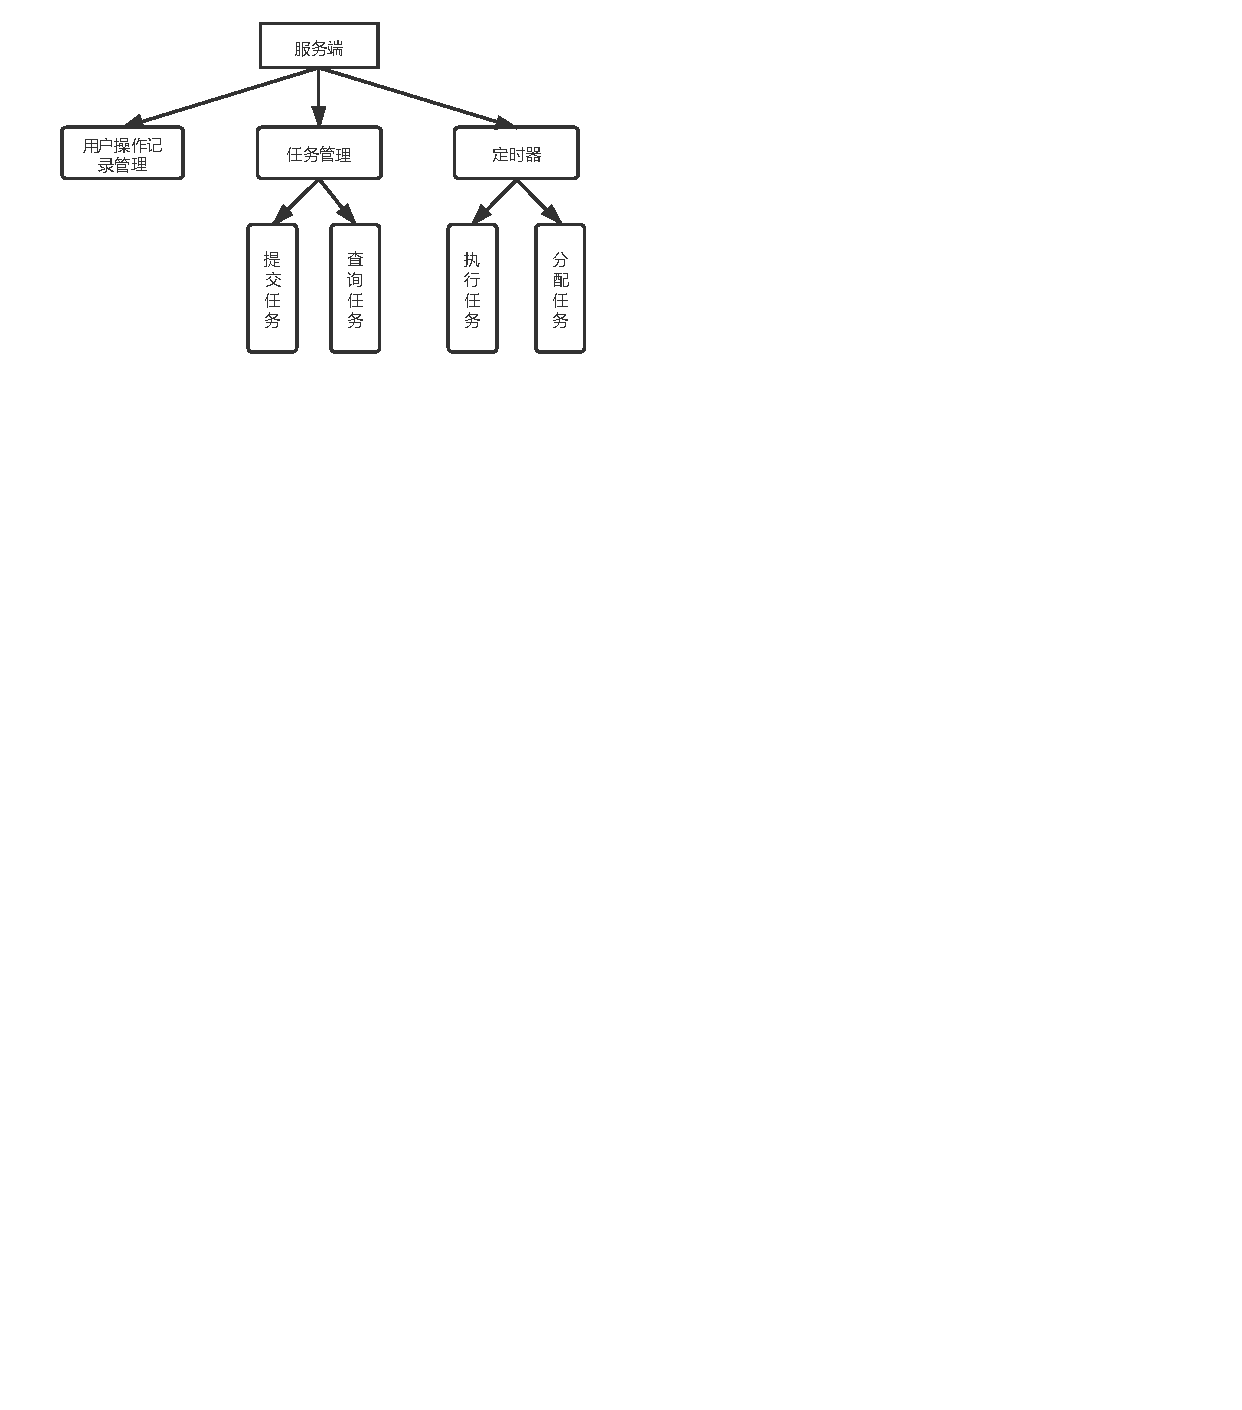
\includegraphics[width=12cm]{images/server.pdf}
    \caption{服务端主要模块设计}
    \label{fig:server}
\end{figure}


\subsection{用户操作记录管理}
为了方便后续的数据分析,我们需要采集用户的所有用户操作记录。客户端通过调用服务端接口将用户操作记录保存在数据库中,用户操作记录的数据库表的主要字段如表 \ref{tab:op_log} 所示:

\begin{table}[]
    \centering
    \begin{tabular}{lll}
        \toprule
        字段 & 类型 & 描述 \\ 
        \midrule
        id & int & 主键 \\
        user, & text & 用户唯一标识 \\ 
        device & text & 所用设备信息 \\
        op & text & 操作名 \\
        info & text & 操作信息 \\
        createTime & datetime & 创建时间 \\
        updateTime & datetime & 更新时间\\
        \bottomrule
    \end{tabular}
    \caption{用户操作记录表}
    \label{tab:op_log}
\end{table}


其中,user字段用于标识用户,默认使用用户手机号作为唯一标识,要求用户进入系统前需要通过手机验证码进行登录。


而在后续的实验环节,为了方便用户跳转完成问卷,不需要用户进行登录,user字段采用的是wjx-问卷星id。

\begin{figure}[ht]
    \centering
    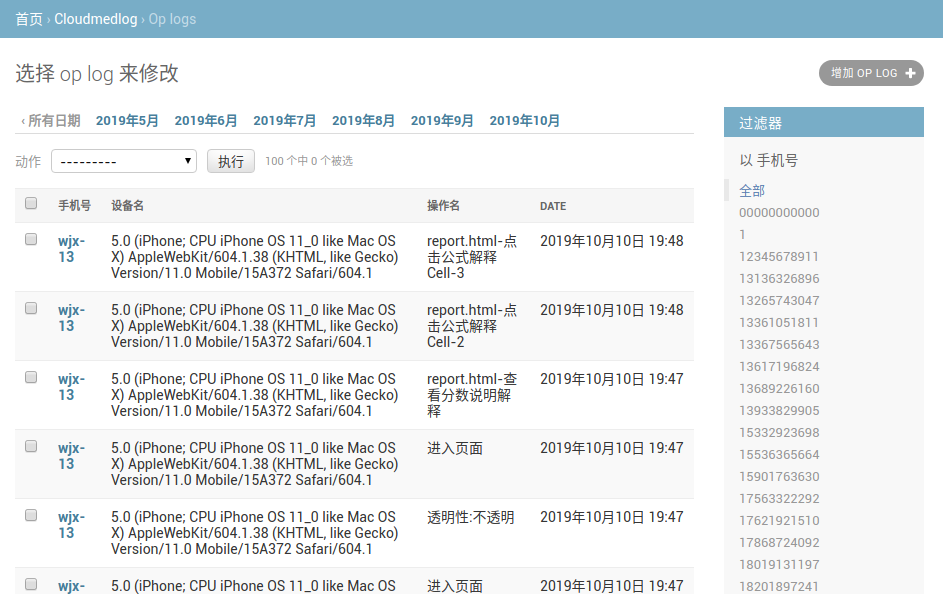
\includegraphics[width=12cm]{images/op_log.png}
    \caption{用户操作记录管理界面}
    \label{fig:op_log}
\end{figure}

\subsection{第三方问卷关联}
每次实验之前,根据实验的需求,可能需要先让用户填写一个问卷,收集必要的用户信息或者对用户进行评测;同样,在实验结束之后,也需要让用户填写问卷,收集用户反馈等。
在服务端重新实现问卷系统增加了工作量,我们通过接入第三方的问卷系统来实现,因此本系统需要对第三方的问卷系统提供对应的支持。


\begin{figure}[h]
    \centering
    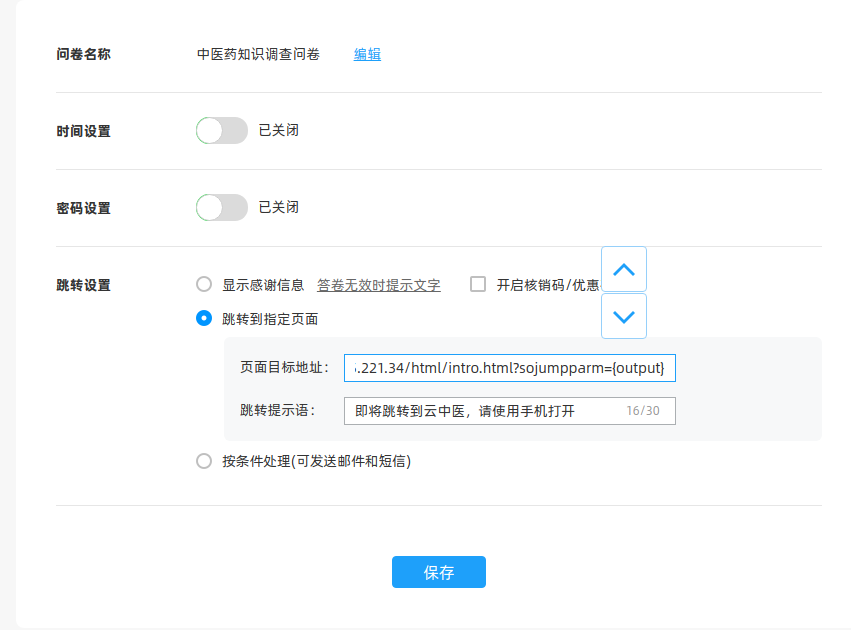
\includegraphics[width=10cm]{images/wjx1.png}
    \caption{第三方问卷系统跳转}
    \label{fig:wjx-ssojump}
\end{figure}

一次大致的实验流程为: 填写实验前问卷->进入实验平台完成实验->填写反馈问卷。在这个过程中,为了方便用户,我们需要通过特定的地址参数完成从问卷到实验平台完成自动登录。

如图\ref{fig:wjx-ssojump}所示,以问卷星为例,企业版的问卷星用户支持问卷完成后跳转到指定地址。指定的地址中可以带模板变量,如问卷的唯一id。
因此我们在系统登录页上只要判断是否存在该变量,如果存在则新建一个平台缩写+唯一id的用户名完成自动登录。


\subsection{任务处理}
一次用户诊断,服务端需要完成多个任务,目前支持的任务可以大致分类两类,计算任务和诊断任务。


\subsubsection{计算任务}
\begin{table}[]
    \centering
    \begin{tabular}{lll}
        \toprule
        字段 & 类型 & 描述 \\ 
        \midrule
        id & int & 主键 \\
        type, & int & 任务类型: 面部,舌部,诊断, 合并 \\ 
        extra & json & 模型相关信息 \\
        in & text & 任务输入 \\
        out & text & 任务结果 \\
        handler & text & 分配的服务端 \\
        status & int & 任务状态: 新建,已分配,处理中,失败,完成 \\
        createTime & datetime & 创建时间 \\
        updateTime & datetime & 更新时间\\
        \bottomrule
    \end{tabular}
    \caption{任务表}
    \label{tab:task}
\end{table}
计算任务对用户的输入进行计算,背后通过模型池中的模型来完成计算,如:面部特征提取任务,舌部特征提取任务,问诊任务。

服务端在收到用户提交的任务之后,会将数据存储到数据库的task表中,task表的主要字段如表 \ref{tab:task}所示:

\begin{enumerate}
    
    \item type一共有四种取值,目前对应四种任务类型:面部特征提取任务,舌部特征提取任务,诊断任务和合并任务。

    \item in为任务的输入,其中面部特征提取和舌部特征提取任务需要的输入为图片,通过Base64编码序列化为json对象,保存在in字段中。

    \item out为任务的执行结果,在模型池的服务完成计算之后,服务端将任务执行结果保存到out字段,同时更新任务的状态。

    \item  handler保存当前任务是由哪个服务端在负责处理。

    \item extra通过json格式存储模型相关信息,如分类任务,如体质判别,输出的7中体质的中文名称,保存在extra中。
\end{enumerate}

\subsubsection{诊断任务}
% 合并任务只有前置任务,没有后置任务,它是整个任务调度流程中的最后一个任务。合并任务的主要功能是在所有计算类型的任务完成后,对计算出来的结果进行合并。

% 合并任务的触发时机,是在合并任务的所有前置任务完成之后。合并任务的合并流程如下:

诊断任务的执行逻辑在服务端实现,不在模型池中有对应的模型。 诊断算法的输入为每个任务的结果,输出为体质得分,健康分数。

在各类任务完成之后,诊断任务通过从redis或者mysql中获取当前已完成任务的结果作为输入,完成最终的诊断。 
诊断任务的内部实现是有一套规则系统组成,定义了每一个任务的输入,会对最终的输出产生怎么样的影响。

在该模式下,本地系统可以比较方便的添加新的模型: 在一个新的模型添加之后,只需要在规则系统中,添加一条新的规则即可完成模型的接入。

诊断流程具体如图 \ref{fig:sketch} 所示:

\begin{figure}[ht]
    \centering
    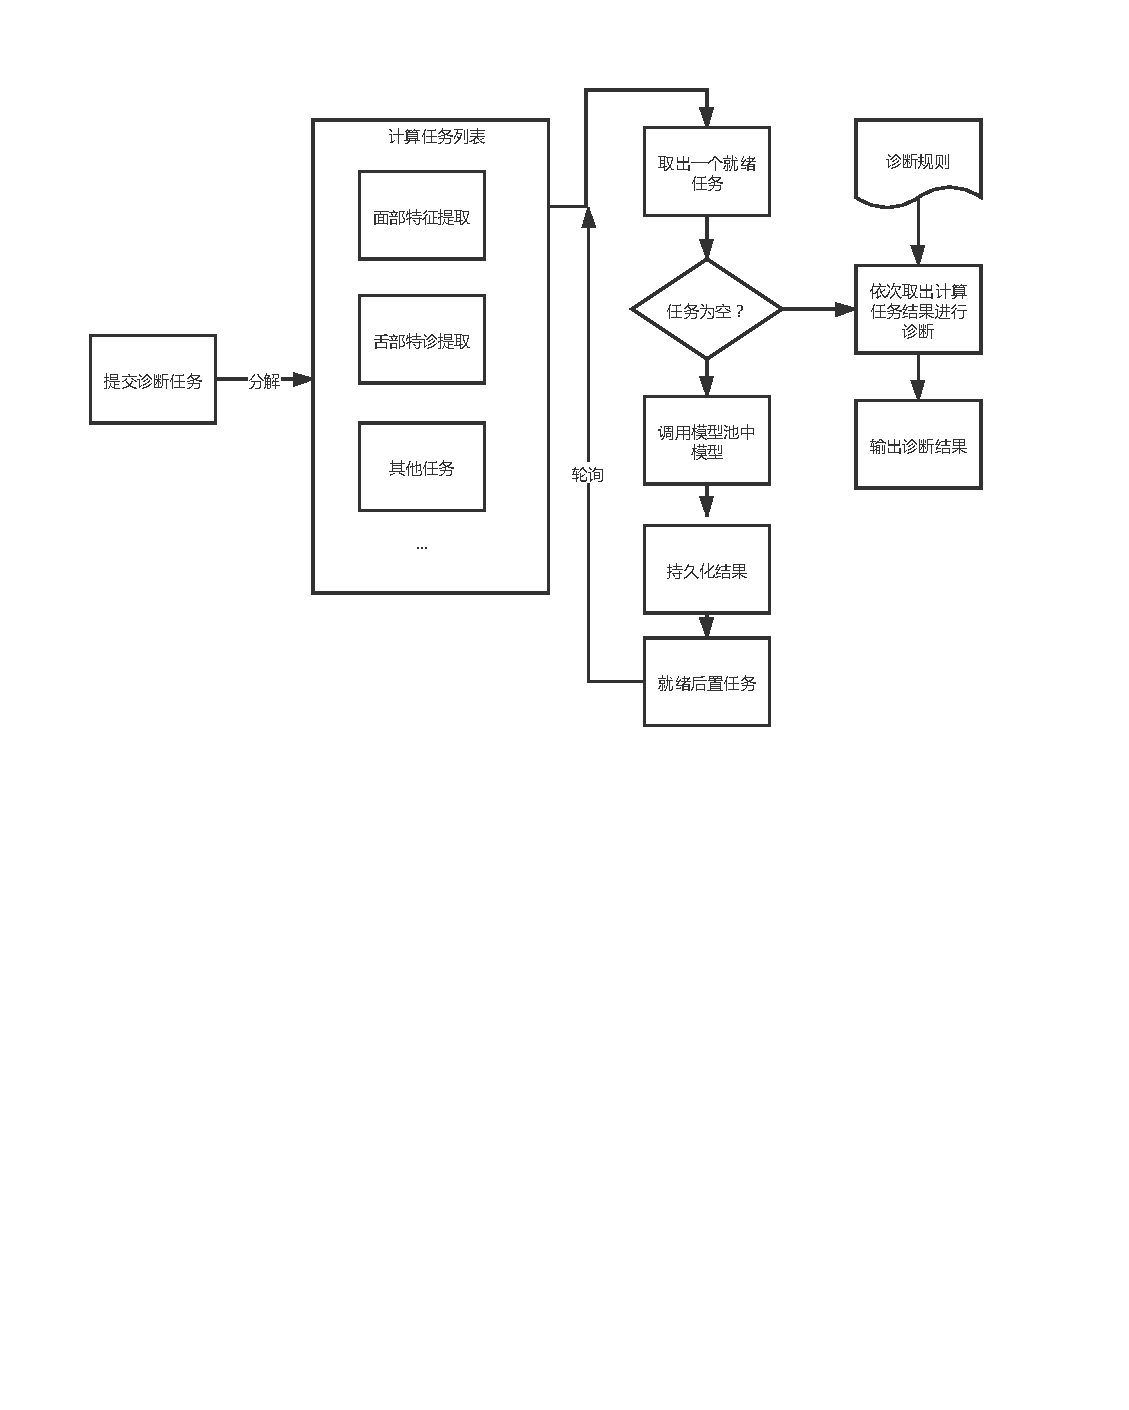
\includegraphics[width=12cm]{images/sketch.pdf}
    \caption{诊断流程}
    \label{fig:sketch}
\end{figure}

用户在提交诊断任务之后,服务端会将诊断任务分解成多个小的计算任务,其中包括面部特征提取,舌部特征提取以及其他相关的任务。任务分解的目的是降低单个服务端实例的计算压力,将任务计算分发到多个服务端,提高计算速度。
同时分解后的任务结果都保存在mysql数据库中,便于后续算法透明性暴露中间结果给用户。
在任务分解之后,通过轮询选出其中一个未完成的任务,调用相关服务完成计算;如果计算任务事先已经完成计算,或者经过轮询已经完成所有的任务,则通过规则系统,取出计算任务的结果进行诊断。



\subsection{任务分配}
%为什么要这样做?
为了实现服务的稳定性,服务端支持同时开启多个实例,即多个服务端同时处理任务。
同时考虑到性能,服务端设计为读写分离的架构:每个实例都可以读取任务列表,处理用户的任务,但只有主节点有任务分配的权限。


\subsubsection{主从节点}
% 为什么要这样做
为了屏蔽用户间的设备差异,让硬件较差的用户设备也能调用模型,本系统采用算法模型和客户端剥离的方案。
模型和客户端剥离则增加了服务端的计算压力,对系统稳定性要求更高。
因此服务端通过实现简单的读写分离和主从竞选的机制,使得服务端支持同时运行多个实例,提高稳定性和性能。


为了实现服务端的高可用,本文将服务端设计成允许多个实例同时运行,如果不做主从节点划分的话,每次有可用的任务时,所有节点都去抢占任务,会有大量锁的竞争的问题。
因此本文将每个实例的角色划分为主节点和从节点进行读写分离,不同节点的具体职责如下:

\begin{enumerate}
    \item 主节点: 通过任务的id进行哈希,按照哈希进行任务的分配给各个节点,更新task表。分配任务时,只有主节点才有对任务表进行写操作的权限。

    \item 从节点: 每个从节点每过一定的间隔时间,就会去读取任务列表,开始执行任务列表里属于自己的任务。  

\end{enumerate}

这样就保证了任务分配只由主节点去更新task表,而执行任务时,每个节点只会执行分配给自己的任务。

\subsubsection{角色竞选流程}
\begin{figure}
    \centering
    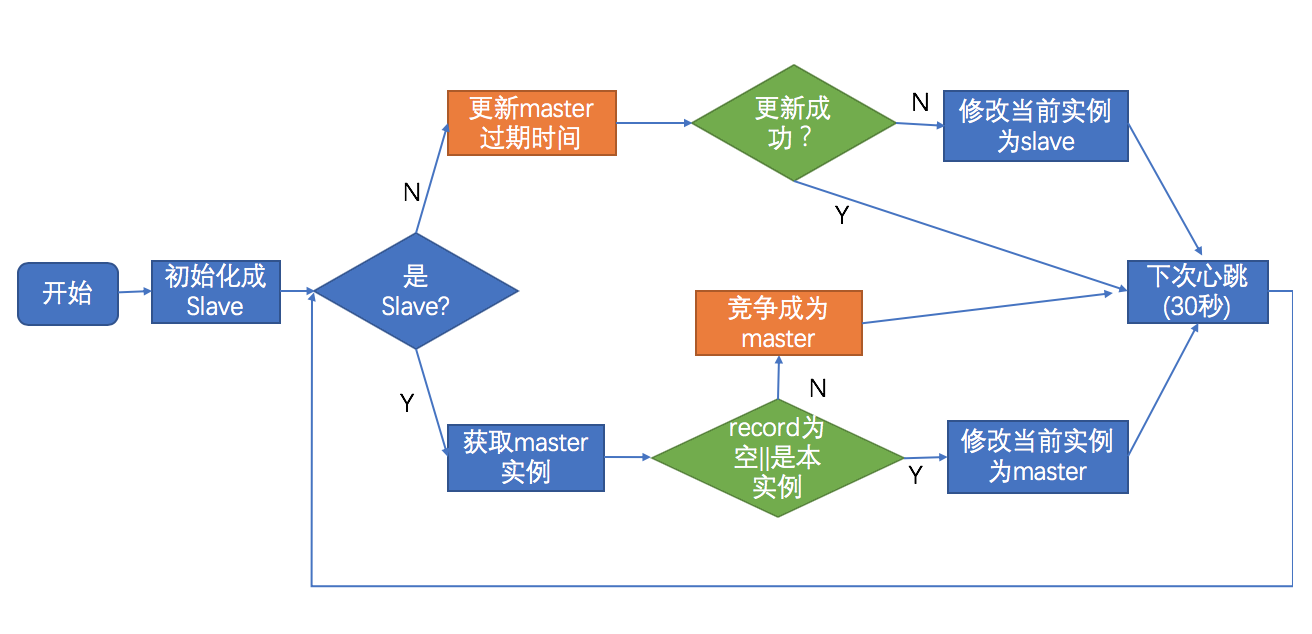
\includegraphics[width=10cm]{images/slave-master.png}
    \caption{服务端角色竞选}
    \label{fig:slave_master}
\end{figure}

服务端通过主从节角色分配的方式,同时运行多个实例来提高系统的响应速度,但多个实例同时运行也带来了系统稳定性的问题,如节点因为网络问题或者其他问题失效时,则需要通过心跳包探测节点存活。

服务端通过心跳包探活,主节点失效时,通过redis的分布式锁实现主节点的竞选。

每个节点在启动之后,会在本地把自己的角色默认设置成从节点。
然后每过一段时间,判断自己节点的类型,主从节点分别执行以下的心跳策略竞选主节点:

\begin{enumerate}
    \item 主节点:主节点每次心跳的时候,更新redis中主节点的过期时间。如果更新成功,等待下一次心跳; 如果更新失败(更新失败可能是自己没有及时更新,导致redis里的主节点过期,主节点的身份被其他节点竞争到了),则把自己的节点类型设置成从节点。
    
    \item 从节点:从节点每次从redis里获取主节点的信息,如果主节点信息无效或者长时间没有心跳(默认设置为两轮心跳周期),则开始抢占竞选锁,尝试更新redis的信息让自己成为主节点;如果redis的主节点信息已经是本节点,说明上一轮抢占成功,将本节点的角色更新为主节点。 
\end{enumerate}



\section{本章小结}
本章介绍了实验平台的方案选型到具体实现,其中实验平台被划分为模型池、服务端和客户端。
这样,客户端就与模型以及诊断细节实现了独立,只需要关注交互的部分。同时为了方便实验,服务端还提供了用户操作记录管理和问卷关联的功能,方便采集用户信息和后续分析用户行为。
客户端的具体实现和实验内容密切相关,不同的实验中客户端的具体实现不同,所以客户端的内容在下一章具体介绍。
